\chapter{\textit{Trabalhos Relacionados}}
	\label{ch:trabalhos}
Nesta seção será comentado sobre alguns trabalhos que possuem um objetivo similar ou utilizam tecnologias similares a este. 

O trabalho de \cite{gprsTelemetrySystem2013} propõe uma solução de telemetria para um veiculo de competição elétrico. A proposta é similar a do trabalho proposto no quesito de manter a equipe em questão atualizada dos dados provindos do carro, a diferença é que o veículo é movida a energia limpa, elétrica. Este requisito altera também a algumas das grandezas a serem analisadas pelo sistema, nele são verificados fatores como amperes por hora, voltagem, velocidade e distancia percorrida. Infelizmente o trabalho não comenta como é feita a coleta dos dados pelos sensores, apenas comentando que existe um equipamento que faz o mesmo. Para parte de telemetria, os desenvolvedores comentam que trabalharam com foco em resolver dois problemas: Robustez sobre todo o circuito de provas e segurança dos dados, além de redução do ruído. Portanto duas tecnologias foram analisadas para a transmissão dos dados embarcados do veículo até os computadores da equipe, a de radio frequência e a rede móvel de celular (GSM). A ultima foi escolhida devido a "(...) Impossibilidade de garantir a comunicação entre todos os circuitos devido aos formatos e obstáculos encontrados no terreno...", também é comentado que foram realizados testes e todos os circuitos possuem cobertura de sinal móvel. Por ultimo é desenvolvido um \textit{software} para receber os dados provenientes do veículo. O sistema de aquisição de dados teve seu funcionamento dividido em quatro blocos, sendo eles: Configuração do aplicativo e do canal transmissão de dados usado; Informações específicas da direção do piloto e do circuito percorrido; Valores numéricos dos dados técnicos mais importantes para a manutenção do veículo em tempo real; Representação gráfica de toda a informação recebida durante todo o processo da prova. Com isto e o tratamento das informações, o programa apresenta para a equipe de boxes informações como:

\begin{itemize}
	\item Consumo de energia; 
	\item Voltagem da bateria;
	\item Velocidade;
	\item Distância percorrida;
	\item Eficiência energética; 
\end{itemize}

Todas estas informações disponíveis são muito interessantes, porém \cite{gprsTelemetrySystem2013} não se aprofunda na sua construção, o que poderia aumentar em muito a relevância deste trabalho para o projeto proposto. Como é comentado, existe um indício de emprego de técnicas de engenharia de \textit{software} na criação do sistema de aquisição de dados, porém por não ser o foco do trabalho, as mesmas não são citadas. 

Outro trabalho que também possui um carro movido a energia limpa e propõe um sistema de aquisição de dados é \cite{applicationOfData2010}. O sistema é feito para um carro que utilizada um motor elétrico e deve ser capaz de percorrer distâncias de mais de 3000 quilômetros no evento \textit{World Solar Challenge}. Os equipamentos utilizados pela equipe foram o CompactRIO e LabVIEW da \textit{National Instrument}, para aquisição dos dados e a criação da plataforma de tratamento de dados, respectivamente, além do modulo de transmissão por radio frequência \textit{MaxStream} (atualmente \textit{Digi}) \textit{Xtream}. Como todos os dispositivos usados pela equipe são feitos por uma fabricantes externos, pouco é discutido sobre como funciona os sensores. O artigo demonstra um pouco sobre a arquitetura do sistema montado, utilizando os equipamentos citados e fala dos resultados, também não comentando muito sobre como foi feita a abordagem de criação do \textit{software} e que requisitos ele deve suprimir. Um dado interessante visto neste artigo é que para coletar dados de seis termopares, dois transdutores, um grupo de bateria e um tacômetro, foi necessário $363,3$ kilobytes de dados por hora, assim um cartão SD de dois gigabytes seria suficiente para armazenar uma longa bateria de treinos.

O artigo \cite{racecarInstrumentationFor2012} é mais abrangente, ele utiliza de um sistema de aquisição de dados e telemetria para estudar o comportamento de motoristas ao volante de carros convencionais. O estudo de comportamento visto no artigo não é verificado por não ser o foco, porém a parte de instrumentação faz algumas menções muito interessantes. Os testes feitos para as analises de dirigibilidade possuem alguns sensores construídos pelos autores, como o de posição do acelerador e sensores para cada roda a fim medir sua velocidade individual (útil em casos de derrapagem), e outra parte dos dados são pegos com um equipamento chamado \textit{Racelogic} VBOX, ele tira alguns dados como aceleração de 0 a 100 e distância percorrida utilizando GPS. Para as entradas analógicas foi comprado um sistema de aquisição de dados da \textit{National Instruments} modelo USB-6211 USB M Series (ou, como é chamado no artigo, NI-DAQ), onde tais entradas eram direcionadas a ele. Para os sensores de velocidade das rodas foi utilizado uma placa de prototipagem AVR-P40-USB-8535 da \textit{Olimex} em conjunto com um microcontrolador \textit{Microchip} da família ATMega32. O \textit{software} criado tem um codigo feito na linguagem C/C++, e o programa tem como objetivo se comunicar com a placa de prototipagem AVR e o sistema de aquisição de dados NI-DAQ, além de outros periféricos citados no texto do artigo. Tendo essas informações, o \textit{software} trata elas e disponibiliza para o usuário em tempo real, além de armazenar os dados em um arquivo de texto para análises posteriores. O \textit{software} tem taxa de atualização de 100 Hz, sendo a taxa de amostragem do NI-DAQ de 100Hz e a taxa de amostragem do sensores de roda de 20Hz no qual o valor final mostrado ao usuário é o ultimo dado recebido dos sensores. O artigo apresenta um diagrama, esquematizando o funcionamento do \textit{software}, e além da parte de sensoriamento ainda existem os algoritmos criados para o estudo de comportamento, aumentando o nível de complexidade total do sistema. Apenas o diagrama não seria suficiente para manter a equipe de desenvolvimento atualizada do progresso do \textit{software} proposto, mas como o foco do texto não esta na engenharia de \textit{software}, esta parte não se encontra discutida por completo.


Outro artigo revisado foi \cite{vehicleDataAcquisition2014}, este traz uma solução de aquisição de dados com um SCOB customizados para Formula SAE, porem o sistema é de uso geral na área veicular, podendo ser instalado em quaisquer outros modelos. O artigo não é muito específico em como e quais sensores são usados, ele coloca alguns exemplos como um sensor para temperatura (LM35) e como é feito um filtro matemático a partir da mediana de 100 valores para obter um resultado mais confiável. O foco do artigo é na parte de telemetria, nesta área é discutido uma solução para qual protocolo \textit{wireless} utilizar para o fim sensoriamento veicular. Algumas opções são descartadas no começo, como \textit{Bluetooth} e infravermelho, devido ao alcance limitado e a necessidade de manter contato direto entre os nós, o que é inviável em um circuito automobilístico. Então foram estudados dois outros protocolos, o WiFi e ZigBee. O artigo comenta que ambos possuem alcance mínimo para o cenário, ambos trabalham na frequência 2.4GHz e podem ter seus dados encriptados. Contudo o ZigBee foi escolhido devido a melhor relação de consumo de energia, além de, segundo o autor, ser mais simples de se instalar uma malha de rede ZigBee. A vantagem do WiFi é maiores taxas de transferência, porém no sistema analisado este requisito não era prioritário.         

O artigo brasileiro \cite{projetoMiniBaja2006} traz várias informações sobre o sistema eletrônico do Paraibaja, equipe de baja da Universidade Federal de Campina Grande. O artigo não é focado em telemetria e aquisição de dados, portanto não existe \textit{software} para ser analisado ou coleta de dados, mas este artigo comenta como a equipe fez para montar seu painel de instrumentos, este mesmo possui alguns sensores interessantes, que apesar da data, devem ser levados em consideração. A equipe trabalhou com o velocímetro, tacômetro, termômetro, medidor de nível de combustível e indicador de nível de óleo baixo. Todos esses sensores foram ligados a um microcontrolador AT89S8252 para manipulação dos dados e exibição das medidas no \textit{display} do painel. Para a visualização destas mesmas informações o sistema conta com um \textit{display} de sete segmentos e LEDs indicadores (para RPM e superaquecimento do motor). O artigo então comenta como são utilizados os sensores para retirada de informação, o termômetro por exemplo, utiliza uma sonda de alumínio acoplada ao cárter do motor, mesmo processo utilizado atualmente pela equipe Velociraptor. Essa sonda, além de ser feita de alumínio, também tem seu interior preenchido com pasta térmica, o que garante uma boa condutividade térmica e um medição mais próxima do valor real. Outro dado interessante é que o valor considerado para superaquecimento do motor é 120ºC, caso este valor seja ultrapassado, um LED indicativo no painel é acendido para informar o piloto.       

Os artigos \cite{designAndImplementation2015} e \cite{developmentOfAn2016} são do mesmo autor no qual \cite{developmentOfAn2016} é desenvolvido um sistema de analise de comportamento na direção em cima de uma plataforma de aquisição de dados e \cite{designAndImplementation2015} é um artigo focado na construção da plataforma utilizada, sendo este o foco deste trabalho. Este sistema de aquisição de dados e monitoramento com telemetria foi especificamente feito para carros convencionais, pois ele utiliza uma entrada de leitura de dados padrão na maioria dos carros convencionais de rua. A \textit{On-Board Diagnostics} (Figura \ref{fig:obd}) é uma entrada presente geralmente na parte inferior do painel dos veículos e fornece informações diretamente da ECU do mesmo. Além de ser uma entrada padrão, os protocolos de interfaceamento para a retirada dos dados também são padronizados e independente de montadora, sendo está porta muito utilizada em oficinas para retirada de diagnósticos preliminares do veículo. Além desta fonte de informações, o autor também utiliza de um sensor de movimento MPU6050 para medir aceleração lateral e velocidade angular. Todos estes dados são enviados para um SCOB que diferente da maioria dos outros artigos aqui citados, consiste em um \textit{Raspberry Pi}. Isto é importante pois o artigo cita algumas vantagens interessantes de se ter uma \textit{PC Board} para processamento dos dados recebidos. Uma das vantagens é o poder de processamento superior em relação a um microcontrolador o que dependendo dos requisitos do projeto pode ser fundamental. Outra vantagem é a possibilidade de utilização de linguagens interpretadas como Python e Ruby, tudo graças ao ambiente que suporta um sistema operacional completo. Uma ultima vantagem comentada é a possibilidade de uso de um sistema gerenciador de bancos de dados integrados com o SCOB para \textit{backup} de informações e otimização do uso de memoria para armazenamento de dados, além de aumento na confiabilidade dos dados. Porém uma desvantagem que não é levantada mas deve ser levada em consideração é o aumento do custo monetário do projeto, com o preço de um \textit{Raspberry Pi} sendo aproximadamente dez vezes o preço de um \textit{Arduino Nano} (Novembro de 2017). O \textit{software} desenvolvido para este projeto utiliza \textit{Labview} e funciona via internet com uma interface web. Os dados são guardados dentro do SCOB e quando requisitado pelo computador são baixados, caso o computador não consiga fazer o carregamento das informações do SCOB, ele utiliza os dados presentes no servidor local. Existe um sistema de usuários para controle das informações e os dados dos sensores são divididos em categorias e podem ser visualizados em tabelas e gráficos. Nos testes, a taxa de amostragem de dados foi fixada em 100Hz e é comentado no artigo que o gargalo do sistema nesse quesito é o sistema \textit{On-Board Diagnostics}, que varia de carro para carro. Não é comentado nenhum tipo de planejamento ou analise de requisitos na parte do \textit{software} e também não é apresentado nenhum diagrama explicando o sistema corrente.    

\begin{figure}[!htb]
	\centering
		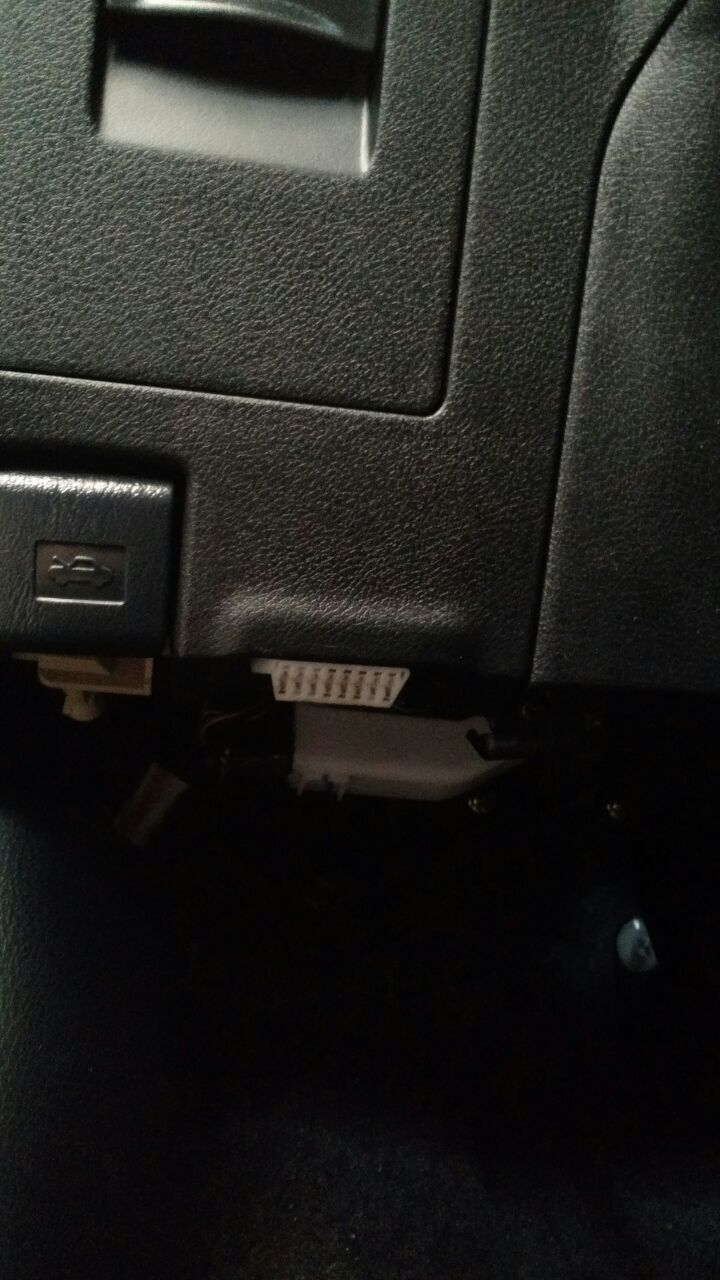
\includegraphics[height=6cm]{obd}
		\caption{Exemplo de entrada \textit{On-Board Diagnostics}. Fonte: Autor.}
		\label{fig:obd}
	\end{figure}

Foram encontrados alguns trabalhos com objetivo similar, como \cite{Dias2010} e \cite{Nunes2016} que tem propostas para criação de um sistema de telemetria para a modalidade baja SAE com um cenário muito similar ao denotado neste trabalho de conclusão de curso. \cite{Dias2010} Tem como foco a pesquisa, projeto e execução da parte de \textit{hardware} do sistema de telemetria, deixando a parte de \textit{software} para um segundo trabalho. Já \cite{Nunes2016} utiliza parte do que já foi projetado em outros anos na equipe Car-Kará para projetar um sistema completo de telemtria com duas ECUs, incluindo \textit{software} e \textit{hardware}.  

